\begin{enumerate}[label=\thesubsection.\arabic*.,ref=\thesubsection.\theenumi]
	\item Determine the loop currents in 
    \figref{fig:ckt1}. 
		\begin{figure}[H] 
    \centering
    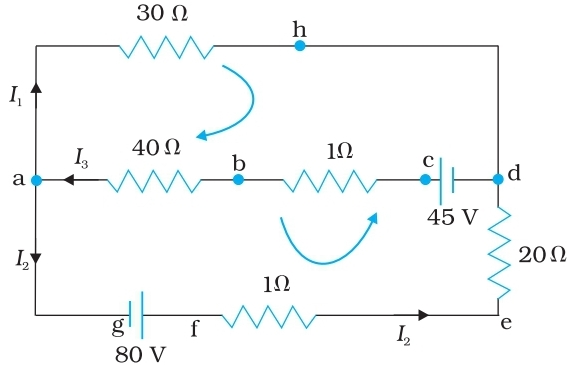
\includegraphics[width=\columnwidth]{figs/ckts/ckt1.jpg} % Adjust width or use height
    \caption{} 
    \label{fig:ckt1} 
\end{figure}
	\item Determine the current in each branch of the network shown in 
    \figref{fig:ckt2}. 
		\begin{figure}[H] 
    \centering
    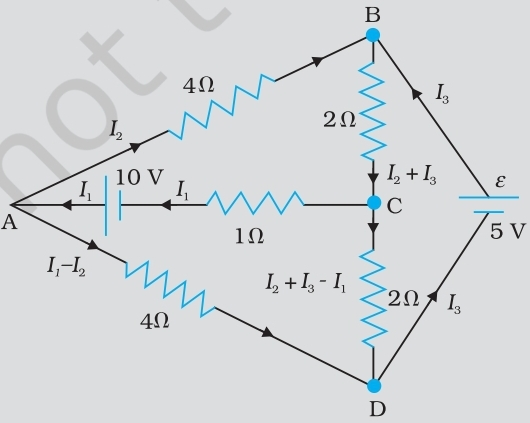
\includegraphics[width=\columnwidth]{figs/ckts/ckt2.jpg} % Adjust width or use height
    \caption{} 
    \label{fig:ckt2} 
\end{figure}
	\item In \figref{fig:ckt3}, a galvanometer of $15\ohm$ resistance is connected across BD. Calculate the current through the galvanometer when a potential difference of $10 V$ is maintained across AC.
		\begin{figure}[H] 
    \centering
    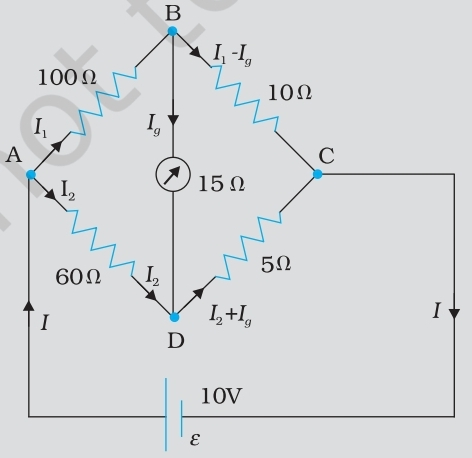
\includegraphics[width=\columnwidth]{figs/ckts/ckt3.jpg} % Adjust width or use height
    \caption{} 
    \label{fig:ckt3} 
\end{figure}
	\item Determine the current in each branch of the network shown in 
\figref{fig:ckt4}.
		\begin{figure}[H] 
    \centering
    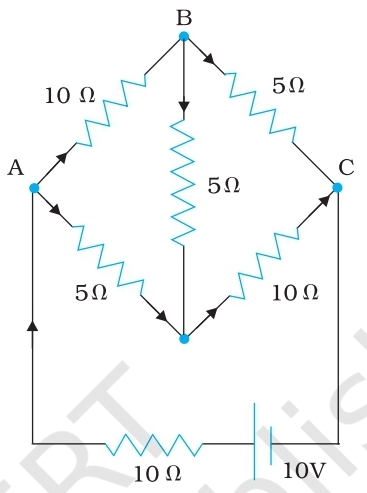
\includegraphics[width=\columnwidth]{figs/ckts/ckt4.jpg} % Adjust width or use height
    \caption{} 
    \label{fig:ckt4} 
\end{figure}
\end{enumerate}
 

